\section{Indledning}
Projektets omhandler behandling af lyd, objektorienteret programmering samt en brug af datakommunikation og softwareudvikling.

To bærbare computere skal kommunikere med hinanden ved hjælp af lyd, hvortil der blev udleveret 2 sæt mikrofoner og højtalere.
Der skal bruges DTMF toner til kommunikationen. Hvilket har har været brugt i gamle telefoner til transmission af telefonnumre over telefonnettet. DTMF står for Dual Tone Multiple Frequency, hvilket betyder at der ligger to toner oven i hinanden med forskellig frekvens, f.eks afspilles tone 1, vil dette indebære frekvenserne 679 Hz og 1209 Hz. \footnote{Digital Signal processing, kapitel 8.11}.

\begin{figure}[h]
\centering
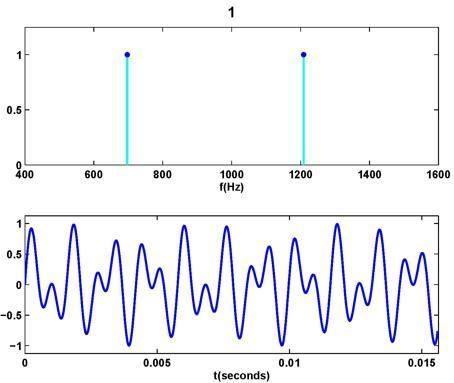
\includegraphics[scale=0.5]{Billeder/DTMF1.JPG}
\caption{DTMF tone 1}
\label{fig:DTMF1}
\end{figure}

Projektet skal skrives i programmeringssproget C++ som er et objektorienteret sprog, samtidig skal software arkitekturen være lagdelt, eksempelvis et fysisk lag og et datalinklag.
Programmet som udvikles skal som krav udføre noget meningsfyldt, så som en styring til en legetøjs bil, eller understøttelse af et multiplayer spil.  